\documentclass[11pt,a4paper]{article}

\usepackage[margin=2.2cm]{geometry}
\usepackage[T1]{fontenc}
\IfFileExists{lmodern.sty}{\usepackage{lmodern}}{}
\usepackage{amsmath,amssymb}
\usepackage{booktabs}
\usepackage{float}
\usepackage{needspace}
\usepackage{array}
\usepackage{enumitem}
\usepackage{xcolor}
\usepackage{listings}
\usepackage{tikz}
\usetikzlibrary{arrows.meta,positioning,calc,shapes.geometric,fit}
\usepackage[most]{tcolorbox}
\usepackage[colorlinks=true,linkcolor=blue!50!black,urlcolor=blue!50!black]{hyperref}
\usepackage{fancyhdr}

\setlength{\parindent}{0pt}
\setlength{\emergencystretch}{2em}
\setlength{\parskip}{6pt}
\renewcommand{\arraystretch}{1.25}

\pagestyle{fancy}
\fancyhf{}
\lhead{\small Video transcript -- Writing your first SDT}
\rhead{\small Compiler Construction}
\cfoot{\thepage}

% ---------- macros ----------
\newcommand{\at}[2]{\ensuremath{#1.\mathit{#2}}}
\newcommand{\tok}[1]{\ensuremath{\mathtt{#1}}}
\newcommand{\inh}[1]{\textcolor{blue!70!black}{#1}}   % inherited
\newcommand{\syn}[1]{\textcolor{red!70!black}{#1}}    % synthesized
\newcommand{\pause}{\textcolor{gray}{\textsf{[pause]}}}

% ---------- boxes for the script ----------
\newtcolorbox{onscreen}{colback=blue!4,colframe=blue!55!black,title={ON SCREEN},fonttitle=\bfseries\small,breakable}
\newtcolorbox{narration}{colback=gray!5,colframe=gray!55,title={NARRATION},fonttitle=\bfseries\small,breakable}
\newtcolorbox{notebox}[1]{colback=orange!6,colframe=orange!75!black,fonttitle=\bfseries\small,title={#1},breakable}

\newcounter{scene}
\newcommand{\scene}[2]{\stepcounter{scene}\needspace{20\baselineskip}\section*{Scene \thescene: #1 \hfill {\normalfont\small #2}}}

\lstdefinestyle{tac}{
  basicstyle=\ttfamily\footnotesize,
  frame=single,
  backgroundcolor=\color{gray!8},
  rulecolor=\color{gray!60},
  columns=fullflexible,
  keepspaces=true,
  xleftmargin=4pt,
  xrightmargin=4pt,
  aboveskip=4pt,
  belowskip=4pt,
  tabsize=4
}
\lstset{style=tac}

\title{\textbf{Writing Your First SDT}\\[4pt]\large A Calculator That Also Counts Its Operations\\[6pt]\normalsize Video transcript}
\author{}
\date{}

\begin{document}
\maketitle
\thispagestyle{fancy}

\begin{notebox}{About this script}
\textbf{Goal of the video.} Students should leave with a \emph{method} for writing an SDT, not with a memorised answer. We derive the SDT for one small grammar in seven steps; the same steps work for any L-attributed grammar.

\textbf{Format.} Each scene has an \textsf{ON SCREEN} box (what the viewer sees) and a \textsf{NARRATION} box (what the speaker says). Words in square brackets are directions to the speaker. The figures are drawn so that they can be built up step by step (the arrows appear one at a time, in the order of the narration).

\textbf{Running time.} About 16 minutes of narration (roughly 2\,300 words at 140 words per minute). With the pauses marked in the script and the step-by-step build-up of the figures, plan for 18 to 20 minutes. The times below are for the narration only.

\begin{center}
\small
\begin{tabular}{@{}c l l@{}}
\toprule
\textbf{Scene} & \textbf{Content} & \textbf{Time} \\ \midrule
1 & The goal and the grammar & 1:20 \\
2 & Step 1: draw the parse tree & 1:25 \\
3 & Step 2: think like a pocket calculator & 1:40 \\
4 & Step 3: who tells whom? (why the grammar is L-attributed) & 1:45 \\
5 & Step 4: inherited or synthesized? & 1:20 \\
6 & Step 5: the dependency graph of the total & 1:45 \\
7 & Step 5 continued: the dependency graph of the counter & 1:15 \\
8 & Step 6: one rule per arrow (the SDD) & 1:35 \\
9 & Step 7: place the actions (the SDT) & 1:25 \\
10 & The same SDT in C & 1:45 \\
11 & Recap: five questions for any SDT & 1:30 \\ \bottomrule
\end{tabular}
\end{center}
\end{notebox}

%====================================================================
\scene{The goal and the grammar}{narration about 1:20}

\begin{onscreen}
Title card: \emph{Writing Your First SDT}. Then the grammar, one production at a time:
\[
\begin{aligned}
E &\to T\,R \\
R &\to +\,T\,R \\
R &\to -\,T\,R \\
R &\to \epsilon \\
T &\to \text{num}
\end{aligned}
\]
Beside it, a window with the input \texttt{9 - 5 + 2} and the wanted output:
\begin{center}
\begin{tabular}{|l|}
\hline
\texttt{Result     = 6}\\
\texttt{Operations = 2}\\ \hline
\end{tabular}
\end{center}
\end{onscreen}

\begin{narration}
Hello everyone, and welcome. Today we are going to write a \emph{syntax-directed translation}, an SDT, from scratch. This usually feels like magic the first time. By the end of this video I hope it will feel like a habit.

Here is our grammar. An expression $E$ is a number followed by $R$, and $R$ is either a plus and a number and more $R$, or a minus and a number and more $R$, or nothing at all. You have seen this grammar before: it is the grammar of sums and differences with the left recursion already removed.

Now the task. We want a small calculator that does \emph{three} things. First, it computes the result of the expression. Second, it counts how many operations were performed, that is, how many plus and minus signs there were. Third, it prints both using two simple \texttt{printf} statements. For the input nine minus five plus two we want to see: result six, operations two.

I will not give you the answer. We will \emph{derive} it, step by step, with questions that you can ask for any grammar. \pause\ Let us start.
\end{narration}

%====================================================================
\scene{Step 1: draw the parse tree}{narration about 1:25}

\begin{onscreen}
Figure~\ref{fig:v-parse} builds up, one node at a time, in the order of the narration. The finished tree stays on screen.
\begin{figure}[H]
\centering
\resizebox{0.78\textwidth}{!}{%
\begin{tikzpicture}[
  every node/.style={font=\small},
  nd/.style={inner sep=2pt},
  leaf/.style={inner sep=2pt,font=\small\bfseries}]
 \node[nd] (E)  at (0,0)       {$E$};
 \node[nd] (Ta) at (-3.4,-1.6) {$T$};
 \node[nd] (R0) at (1.6,-1.6)  {$R$};
 \node[leaf] (n9) at (-3.4,-3.2) {num\,(9)};
 \node[nd] (mi) at (-0.6,-3.2) {$-$};
 \node[nd] (Tb) at (1.6,-3.2)  {$T$};
 \node[nd] (R1) at (4.6,-3.2)  {$R$};
 \node[leaf] (n5) at (1.6,-4.8) {num\,(5)};
 \node[nd] (pl) at (3.4,-4.8)  {$+$};
 \node[nd] (Tc) at (5.2,-4.8)  {$T$};
 \node[nd] (R2) at (7.6,-4.8)  {$R$};
 \node[leaf] (n2) at (5.2,-6.4) {num\,(2)};
 \node[nd] (ep) at (7.6,-6.4)  {$\epsilon$};
 \foreach \a/\b in {E/Ta,E/R0,Ta/n9,R0/mi,R0/Tb,R0/R1,Tb/n5,R1/pl,R1/Tc,R1/R2,Tc/n2,R2/ep}
   \draw[gray!70] (\a.south)--(\b.north);
\end{tikzpicture}}
\caption{The parse tree of \texttt{9 - 5 + 2}. Each $R$ holds one operator and one number; the final $R\to\epsilon$ marks the end of the input.}
\label{fig:v-parse}
\end{figure}
\end{onscreen}

\begin{narration}
Step one is always the same: \emph{draw the parse tree of a small example.} Do not skip this step; the tree is where the ideas come from.

We start with $E$. The first production says $E$ becomes $T$ followed by $R$. The $T$ becomes the number nine. [Point to the left branch.] Now the $R$. The next symbol in the input is a minus, so we use $R$ goes to minus, $T$, $R$. That $T$ is the number five. The next $R$ sees a plus, so we use $R$ goes to plus, $T$, $R$, and that $T$ is the number two. Finally the input is finished, and the last $R$ goes to epsilon. \pause

Look at the shape of this tree. It is a long chain of $R$'s going down and to the right. Each $R$ carries exactly \emph{one operator and one number}. And notice what the tree does \emph{not} show: nowhere does it say that nine minus five should be calculated first. The tree just lists the pieces, from left to right.

That is the job of the SDT: to add the \emph{meaning} to this tree. So the question for the next step is: how do we give the tree a memory? \pause
\end{narration}

%====================================================================
\scene{Step 2: think like a pocket calculator}{narration about 1:40}

\begin{onscreen}
A pocket calculator image, and a table that grows row by row:
\begin{center}
\begin{tabular}{@{}c c c c@{}}
\toprule
\textbf{Key pressed} & \textbf{Display} & \textbf{Tally of operations} & \textbf{Tree node} \\ \midrule
\texttt{9} & 9 & 0 & first $R$ starts here \\
\texttt{- 5} & 4 & 1 & second $R$ \\
\texttt{+ 2} & 6 & 2 & third $R$ \\
(no more keys) & \textbf{6} & \textbf{2} & $R\to\epsilon$: the answer \\ \bottomrule
\end{tabular}
\end{center}
\end{onscreen}

\begin{narration}
Let us forget compilers for one minute and use a pocket calculator. You type nine. You press minus five, and the display shows four. You press plus two, and the display shows six. \pause

Think about what you did \emph{not} do. You did not remember the whole expression. You only looked at the display, which shows \emph{the result so far}, and then you applied the next operation to it. That is the whole trick.

Now our calculator has to do one more thing: count the operations. So imagine a piece of paper next to the calculator, where you make one tally mark for every operation. After minus five: one mark. After plus two: two marks.

So we need \emph{two} pieces of memory: the \textbf{running total}, and the \textbf{operations counted so far}.

Now comes the key idea of this video. Look at the table again. Each row corresponds to one $R$ in our tree. So let us give \emph{every $R$ two boxes}: one for the total so far, and one for the number of operations so far. Each $R$ will \emph{read} the two boxes, \emph{update} them with its own operator and its own number, and \emph{hand them on} to the next $R$.

And at the bottom of the tree, at the epsilon? There is nothing left to read, so the display \emph{is} the final answer. Our two boxes hold the result and the operation count. All we have to do is to bring them back up to the top, where the \texttt{printf} is waiting. \pause
\end{narration}

%====================================================================
\scene{Step 3: who tells whom? Why this grammar is L-attributed}{narration about 1:45}

\begin{onscreen}
Figure~\ref{fig:v-zoom}: the production $R\to -\,T\,R_1$ alone. Boxes: $i$ (total so far) and $c$ (count so far) on the left of each $R$; $s$ (final total) and $n$ (final count) on the right. The blue arrows appear one by one.
\begin{figure}[H]
\centering
\resizebox{0.9\textwidth}{!}{%
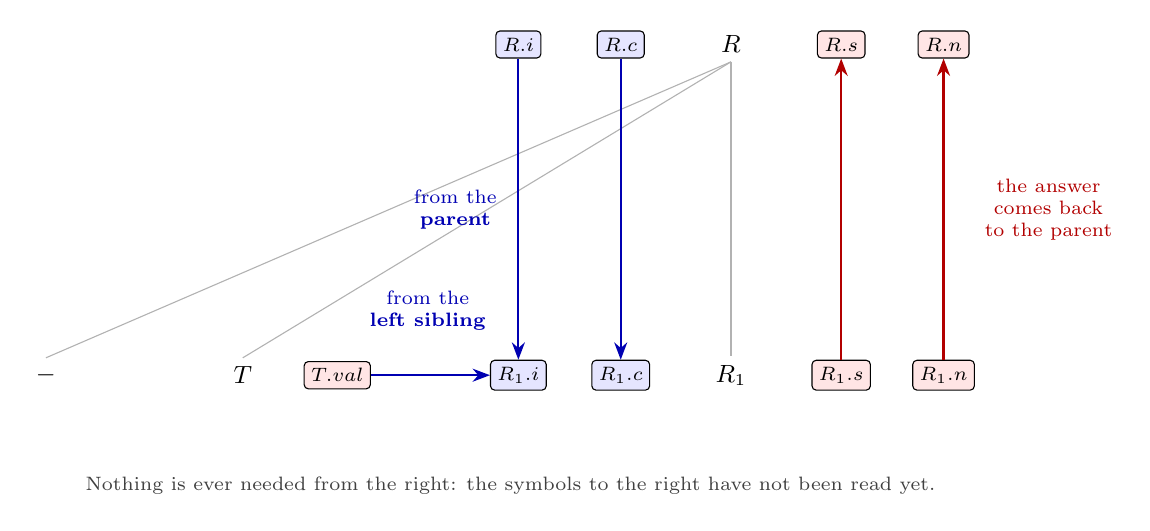
\begin{tikzpicture}[
  every node/.style={font=\small},
  nd/.style={inner sep=3pt},
  ib/.style={draw,rounded corners=1.5pt,fill=blue!10,inner sep=2.5pt,font=\scriptsize},
  sb/.style={draw,rounded corners=1.5pt,fill=red!10,inner sep=2.5pt,font=\scriptsize},
  dn/.style={-{Stealth[length=2.2mm]},blue!70!black,thick},
  up/.style={-{Stealth[length=2.2mm]},red!70!black,thick},
  lab/.style={font=\scriptsize,align=center}]
 % ---- the parent R (above R_1)
 \node[ib] (Ri) at (1.6,0)  {$R.i$};
 \node[ib] (Rc) at (2.9,0)  {$R.c$};
 \node[nd] (R)  at (4.3,0)  {$R$};
 \node[sb] (Rs) at (5.7,0)  {$R.s$};
 \node[sb] (Rn) at (7.0,0)  {$R.n$};
 % ---- the body of R -> - T R_1
 \node[nd] (mi) at (-4.4,-4.2) {$-$};
 \node[nd] (T)  at (-1.9,-4.2) {$T$};
 \node[sb] (Tv) at (-0.7,-4.2) {$T.val$};
 \node[ib] (R1i) at (1.6,-4.2)  {$R_1.i$};
 \node[ib] (R1c) at (2.9,-4.2)  {$R_1.c$};
 \node[nd] (R1)  at (4.3,-4.2)  {$R_1$};
 \node[sb] (R1s) at (5.7,-4.2)  {$R_1.s$};
 \node[sb] (R1n) at (7.0,-4.2)  {$R_1.n$};
 \foreach \a/\b in {R/mi,R/T,R/R1} \draw[gray!60] (\a.south)--(\b.north);
 % ---- blue: what R_1 needs, from above and from the left
 \draw[dn] (Ri.south)--(R1i.north);
 \draw[dn] (Rc.south)--(R1c.north);
 \draw[dn] (Tv.east)--(R1i.west);
 \node[lab,text=blue!70!black,anchor=east] at (1.45,-2.1) {from the\\\textbf{parent}};
 \node[lab,text=blue!70!black,anchor=south] at (0.45,-3.75) {from the\\\textbf{left sibling}};
 % ---- red: the answer climbs back up
 \draw[up] (R1s.north)--(Rs.south);
 \draw[up] (R1n.north)--(Rn.south);
 \node[lab,text=red!70!black,anchor=west] at (7.4,-2.1) {the answer\\comes back\\to the parent};
 \node[lab,text=gray!50!black] at (1.5,-5.6) {Nothing is ever needed from the right: the symbols to the right have not been read yet.};
\end{tikzpicture}}
\caption{One step of the chain, $R\to-\,T\,R_1$. To fill its blue boxes, $R_1$ needs only things that are \emph{above} it (the parent's boxes) or \emph{to its left} (the number in $T$).}
\label{fig:v-zoom}
\end{figure}
\end{onscreen}

\begin{narration}
Let us zoom into one single step of the chain: the production $R$ goes to minus, $T$, $R_1$. Here $R$ is the parent, and $R_1$ is the new $R$ below it. Remember, we want to \emph{fill the boxes of $R_1$}: the total so far and the count so far.

Question number one: where does the \textbf{total so far} for $R_1$ come from? It was in the boxes of the parent $R$. That is above us. [Draw the first blue arrow.]

Question number two: which number do we subtract? It is the five, and the five lives in $T$, which is the sibling standing \emph{to the left} of $R_1$. [Draw the second blue arrow.]

Question number three: the \textbf{count so far}? It was in the parent's box, again from above. [Draw the third arrow.]

Now look at the picture. \emph{Every single input of $R_1$ comes from above or from the left.} Nothing comes from the right. \pause

This is exactly what the letter L means in the term \textbf{L-attributed}: information may flow from the parent and from the siblings to the \emph{left}, but never from the right. And there is a good reason for it. A parser reads the input from left to right. When it works on $R_1$, the things on the right have not been read yet, so they cannot possibly give us any information.

What about the very first $R$, which has no parent $R$? It gets its total from its left sibling $T$, that is, the number nine, and its count starts at zero. So the first $R$ also follows the rule.

Conclusion: \emph{our grammar is L-attributed, and we can write the SDT.} \pause
\end{narration}

%====================================================================
\scene{Step 4: inherited or synthesized?}{narration about 1:20}

\begin{onscreen}
A two-column card, then the table of our attributes with colours:
\begin{center}
\small
\begin{tabular}{@{}p{6.4cm} p{6.4cm}@{}}
\toprule
\textcolor{blue!70!black}{\textbf{Inherited}} & \textcolor{red!70!black}{\textbf{Synthesized}} \\ \midrule
the value comes from the \textbf{parent} or from a \textbf{left sibling}: it arrives from \emph{above} or from the \emph{left} &
the value is computed from the \textbf{children}: it goes \emph{up} to the parent \\ \bottomrule
\end{tabular}
\end{center}
\begin{center}
\small
\begin{tabular}{@{}l l l p{6.0cm}@{}}
\toprule
\textbf{Attribute} & \textbf{Kind} & \textbf{Meaning} & \textbf{Where its value comes from} \\ \midrule
$T.val$ & \syn{synthesized} & the value of a number & from its child, the token \\
$R.i$ & \inh{inherited} & total so far & from the parent and the left sibling \\
$R.c$ & \inh{inherited} & operations so far & from the parent \\
$R.s$ & \syn{synthesized} & final total & from the child $R_1$ \\
$R.n$ & \syn{synthesized} & final number of operations & from the child $R_1$ \\ \bottomrule
\end{tabular}
\end{center}
\end{onscreen}

\begin{narration}
Now we give names to the boxes, and there are two kinds. A one-sentence test will tell you which kind you have. \pause

Ask: \emph{where does the value come from?} If it arrives from the \textbf{parent or from a sibling on the left}, from above or from the left, then it is an \textbf{inherited} attribute. If it is computed from the \textbf{children} and travels \emph{up}, it is a \textbf{synthesized} attribute.

Let us apply the test to our five attributes. $T.val$, the value of a number: it comes from the child, the token. Synthesized. $R.i$, the total so far: it comes from the parent and from the left sibling. Inherited. $R.c$, the operations so far: it comes from the parent. Inherited. And $R.s$ and $R.n$, the final total and the final count: they come from the child $R_1$, going up. Synthesized.

Do you see the pattern? The \emph{total} makes a U-turn. It goes \emph{down} the chain as the inherited attribute $R.i$, and at the epsilon it turns around and comes \emph{up} as the synthesized attribute $R.s$. The count does exactly the same with $R.c$ and $R.n$. Inherited attributes carry the work \emph{in}; synthesized attributes bring the answer \emph{out}. \pause
\end{narration}

%====================================================================
\scene{Step 5: the dependency graph of the total}{narration about 1:45}

\begin{onscreen}
Figure~\ref{fig:v-dep} appears arrow by arrow in the order of the yellow numbers. Colours: grey = token value; \inh{blue} = inherited; \syn{red} = synthesized.
\begin{figure}[H]
\centering
\resizebox{0.98\textwidth}{!}{%
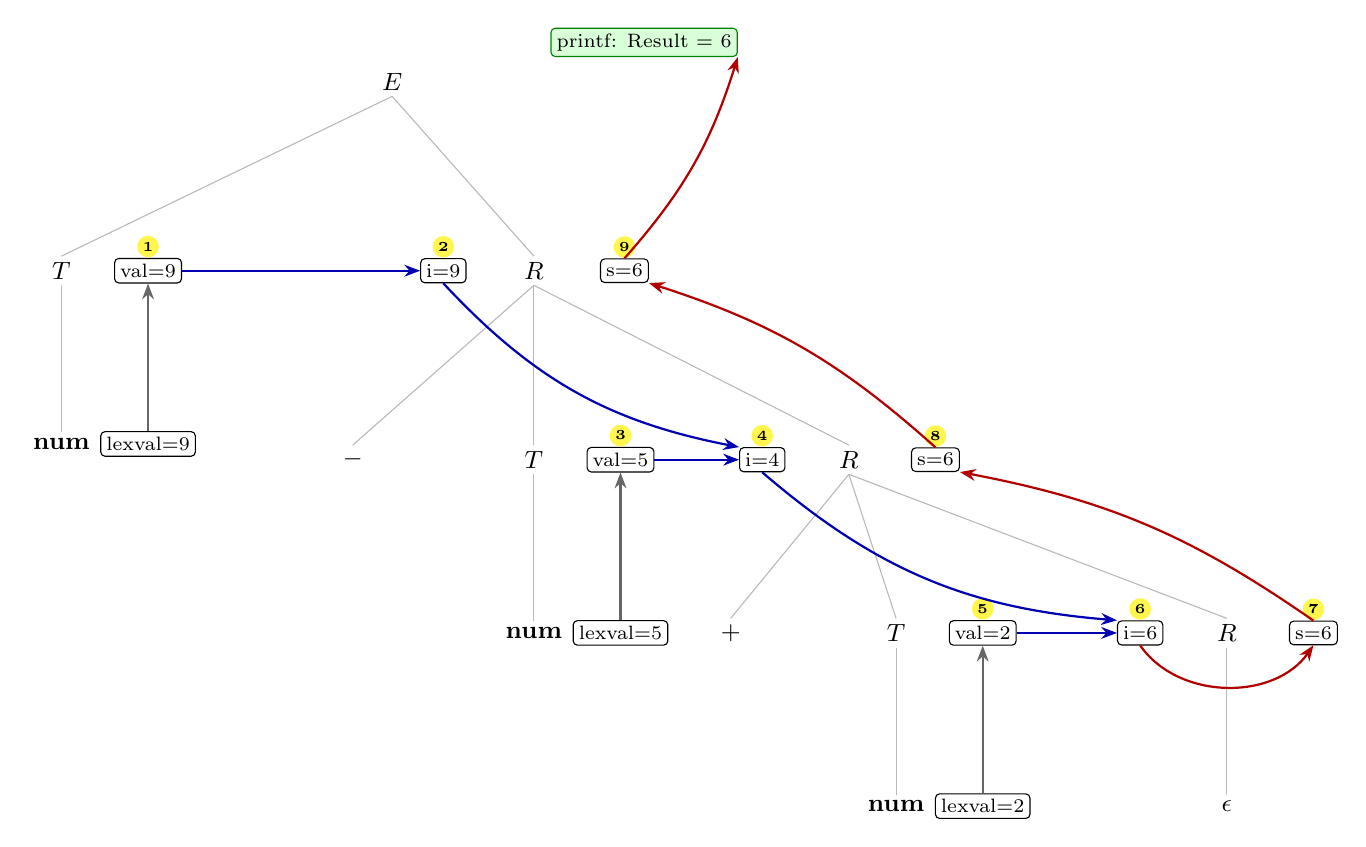
\begin{tikzpicture}[
  every node/.style={font=\small},
  nd/.style={inner sep=2pt},
  ab/.style={draw,rounded corners=1.5pt,inner sep=2pt,font=\scriptsize,fill=white},
  ord/.style={circle,fill=yellow!70,inner sep=1pt,font=\tiny\bfseries},
  tr/.style={gray!55},
  dn/.style={-{Stealth[length=2mm]},blue!70!black,thick},
  up/.style={-{Stealth[length=2mm]},red!70!black,thick},
  lx/.style={-{Stealth[length=2mm]},black!60,thick}]
 % ---- the parse tree
 \node[nd] (E)  at (0,0)       {$E$};
 \node[nd] (Ta) at (-4.2,-2.4) {$T$};
 \node[nd] (R0) at (1.8,-2.4)  {$R$};
 \node[nd] (n9) at (-4.2,-4.6) {\textbf{num}};
 \node[nd] (mi) at (-0.5,-4.8) {$-$};
 \node[nd] (Tb) at (1.8,-4.8)  {$T$};
 \node[nd] (R1) at (5.8,-4.8)  {$R$};
 \node[nd] (n5) at (1.8,-7.0)  {\textbf{num}};
 \node[nd] (pl) at (4.3,-7.0)  {$+$};
 \node[nd] (Tc) at (6.4,-7.0)  {$T$};
 \node[nd] (R2) at (10.6,-7.0) {$R$};
 \node[nd] (n2) at (6.4,-9.2)  {\textbf{num}};
 \node[nd] (ep) at (10.6,-9.2) {$\epsilon$};
 \foreach \a/\b in {E/Ta,E/R0,Ta/n9,R0/mi,R0/Tb,R0/R1,Tb/n5,R1/pl,R1/Tc,R1/R2,Tc/n2,R2/ep}
   \draw[tr] (\a.south)--(\b.north);
 % ---- attribute boxes (yellow number = order of evaluation)
 \node[ab,fill=green!15,draw=green!50!black] (Pf) at (3.2,0.5) {printf: Result = 6};
 \node[ab,label={[ord]above:1}]  (Tav) at (-3.1,-2.4) {val=9};
 \node[ab,label={[ord]above:2}]  (R0i) at (0.65,-2.4) {i=9};
 \node[ab,label={[ord]above:9}]  (R0s) at (2.95,-2.4) {s=6};
 \node[ab] (l9) at (-3.1,-4.6) {lexval=9};
 \node[ab,label={[ord]above:3}]  (Tbv) at (2.9,-4.8)  {val=5};
 \node[ab,label={[ord]above:4}]  (R1i) at (4.7,-4.8)  {i=4};
 \node[ab,label={[ord]above:8}]  (R1s) at (6.9,-4.8)  {s=6};
 \node[ab] (l5) at (2.9,-7.0) {lexval=5};
 \node[ab,label={[ord]above:5}]  (Tcv) at (7.5,-7.0)  {val=2};
 \node[ab,label={[ord]above:6}]  (R2i) at (9.5,-7.0)  {i=6};
 \node[ab,label={[ord]above:7}]  (R2s) at (11.7,-7.0) {s=6};
 \node[ab] (l2) at (7.5,-9.2) {lexval=2};
 % ---- token value -> T.val
 \draw[lx] (l9.north)--(Tav.south);
 \draw[lx] (l5.north)--(Tbv.south);
 \draw[lx] (l2.north)--(Tcv.south);
 % ---- inherited flow
 \draw[dn] (Tav.east)--(R0i.west);
 \draw[dn] (R0i.south) to[bend right=18] (R1i.north west);
 \draw[dn] (Tbv.east)--(R1i.west);
 \draw[dn] (R1i.south) to[bend right=18] (R2i.north west);
 \draw[dn] (Tcv.east)--(R2i.west);
 % ---- turn-around and synthesized flow
 \draw[up] (R2i.south) to[bend right=55] (R2s.south);
 \draw[up] (R2s.north) to[bend right=12] (R1s.south east);
 \draw[up] (R1s.north) to[bend right=12] (R0s.south east);
 \draw[up] (R0s.north) to[bend right=12] (Pf.south east);
\end{tikzpicture}}
\caption{Dependency graph of the \emph{total} for \texttt{9 - 5 + 2}. An arrow $x\to y$ means ``$y$ is computed from $x$''. The yellow numbers are one valid order of evaluation.}
\label{fig:v-dep}
\end{figure}
\end{onscreen}

\begin{narration}
Now we draw the plan on the tree. This picture is called a \textbf{dependency graph}. Every attribute is a little box next to its node, and an arrow from $x$ to $y$ means: \emph{$y$ is computed from $x$.} The value travels along the arrow. Let us follow it together, in the order of the yellow numbers.

[Number one.] The lexer gives us the number nine, and $T.val$ becomes nine. [Number two.] This nine is the left sibling of the first $R$, so the blue arrow carries it into $R.i$. The running total starts at nine. \pause

[Number three.] Next, $T.val$ is five. [Number four.] Now the second $R$ needs \emph{two} things: the total so far from its parent, nine, and the five from its left sibling. Two blue arrows arrive in the box $R_1.i$, and the box now holds nine minus five, which is four. The same happens for the third $R$ [numbers five and six]: four plus two is six.

[Number seven.] Now we have reached the epsilon. There is nothing left to read. So the total is turned around: $R.s$ is simply a copy of $R.i$. Six. [Numbers eight and nine.] And then the red arrows carry the six back up, one $R$ at a time, until it arrives at the root, where our \texttt{printf} is waiting. \pause

Notice two things. First: the blue arrows go down and to the right, the red arrows go up. Second: \emph{no arrow comes from the right-hand sibling.} That is the L-attributed check, and we pass it. \pause
\end{narration}

%====================================================================
\scene{Step 5 continued: the dependency graph of the counter}{narration about 1:15}

\begin{onscreen}
Figure~\ref{fig:v-cnt}: the counter follows the same route, now drawn as a straight chain. The ``+1'' labels appear on the arrows.
\begin{figure}[H]
\centering
\resizebox{0.98\textwidth}{!}{%
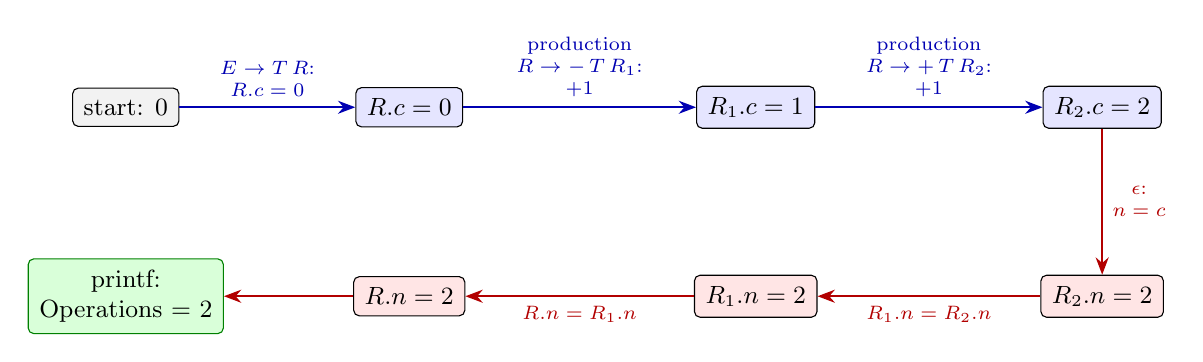
\begin{tikzpicture}[
  box/.style={draw,rounded corners=2pt,inner sep=4pt,font=\small,align=center},
  dn/.style={-{Stealth[length=2.2mm]},blue!70!black,thick},
  up/.style={-{Stealth[length=2.2mm]},red!70!black,thick},
  lab/.style={font=\scriptsize,align=center}]
 \node[box,fill=gray!10] (st) at (-3.6,0) {start: $0$};
 \node[box,fill=blue!10] (c0) at (0,0)    {$R.c=0$};
 \node[box,fill=blue!10] (c1) at (4.4,0)  {$R_1.c=1$};
 \node[box,fill=blue!10] (c2) at (8.8,0)  {$R_2.c=2$};
 \draw[dn] (st)--(c0) node[midway,above,lab] {$E\to T\,R$:\\$R.c=0$};
 \draw[dn] (c0)--(c1) node[midway,above,lab] {production\\$R\to-\,T\,R_1$:\\$+1$};
 \draw[dn] (c1)--(c2) node[midway,above,lab] {production\\$R\to+\,T\,R_2$:\\$+1$};
 \node[box,fill=red!10] (n2) at (8.8,-2.4) {$R_2.n=2$};
 \node[box,fill=red!10] (n1) at (4.4,-2.4) {$R_1.n=2$};
 \node[box,fill=red!10] (n0) at (0,-2.4)   {$R.n=2$};
 \node[box,fill=green!15,draw=green!50!black] (pf) at (-3.6,-2.4) {printf:\\Operations = 2};
 \draw[up] (c2)--(n2) node[midway,right,lab] {$\epsilon$:\\$n=c$};
 \draw[up] (n2)--(n1) node[midway,below,lab] {$R_1.n=R_2.n$};
 \draw[up] (n1)--(n0) node[midway,below,lab] {$R.n=R_1.n$};
 \draw[up] (n0)--(pf);
\end{tikzpicture}}
\caption{The counter travels exactly like the total. The ``+1'' is not computed from another attribute: it happens because the production $R\to\pm\,T\,R_1$ was used.}
\label{fig:v-cnt}
\end{figure}
\end{onscreen}

\begin{narration}
Now the counter. It travels along exactly the same route as the total, so I have drawn it as a straight chain to make it easy to see.

At the start, the rule for $E$ puts a zero into the first $R$. Now look at the arrows between the boxes. Each one carries a \emph{plus one}. And here is something interesting: that \emph{plus one} does not come from any attribute. It comes from the \emph{production} we are using. Every time the parser chooses $R$ goes to plus-$T$-$R$ or $R$ goes to minus-$T$-$R$, an operation has happened. So we add one. \pause

At the epsilon the count is turned around, $R.n$ is a copy of $R.c$, and the two comes back up through the red arrows to the \texttt{printf}.

So our two accumulators, the total and the counter, do exactly the same dance: \emph{down} the chain as inherited attributes, \emph{turn} at the epsilon, \emph{up} the chain as synthesized attributes. If you understand one, you understand both. Here is the whole story in numbers, for each $R$:
\begin{center}
\small
\begin{tabular}{@{}l c c c c@{}}
\toprule
 & $R.i$ & $R.c$ & $R.s$ & $R.n$ \\ \midrule
first $R$ & 9 & 0 & 6 & 2 \\
second $R$ ($R_1$) & 4 & 1 & 6 & 2 \\
third $R$ ($R_2$, then $\epsilon$) & 6 & 2 & 6 & 2 \\ \bottomrule
\end{tabular}
\end{center}
\pause
\end{narration}

%====================================================================
\scene{Step 6: one rule per arrow (the SDD)}{narration about 1:35}

\begin{onscreen}
A two-column table. On the left a question, on the right the rule; each row appears when the speaker reads it. Then the complete SDD on one slide.
\begin{center}
\small
\begin{tabular}{@{}p{5.7cm} p{7.4cm}@{}}
\toprule
\textbf{Question} & \textbf{Semantic rule} \\ \midrule
What is the value of a number? & $\at{T}{val}=\at{\mathbf{num}}{lexval}$ \\
Where does the total start? & $\at{R}{i}=\at{T}{val}$ \hfill (in $E\to T\,R$) \\
Where does the counter start? & $\at{R}{c}=0$ \hfill (in $E\to T\,R$) \\
What happens at a plus? & $\at{R_1}{i}=\at{R}{i}+\at{T}{val}$; \ $\at{R_1}{c}=\at{R}{c}+1$ \\
What happens at a minus? & $\at{R_1}{i}=\at{R}{i}-\at{T}{val}$; \ $\at{R_1}{c}=\at{R}{c}+1$ \\
What happens at the end of the input? & $\at{R}{s}=\at{R}{i}$; \ $\at{R}{n}=\at{R}{c}$ \hfill (in $R\to\epsilon$) \\
How do the answers climb up? & $\at{R}{s}=\at{R_1}{s}$; \ $\at{R}{n}=\at{R_1}{n}$ \\
What do we print? & the values $\at{R}{s}$ and $\at{R}{n}$ of the first $R$, with \texttt{printf} \\ \bottomrule
\end{tabular}
\end{center}
\end{onscreen}

\begin{narration}
Now comes the pleasant part. The rules write themselves, because \textbf{every arrow in the picture is one rule}. We just answer one question per arrow. Let me read them with you.

What is the value of a number? $T.val$ is the lexical value of the token. \pause

Where does the total start? It starts with the number we have just read: $R.i$ equals $T.val$. This is the rule of the production $E$ goes to $T$ $R$. And the counter starts at zero.

What happens at a plus? The new total is the old total plus the number: $R_1.i$ equals $R.i$ plus $T.val$. And the new count is the old count plus one. At a minus, the same, but with a minus sign. \emph{Be careful with the order here}: the old total comes first, $R.i$ minus $T.val$, not the other way around. Subtraction is not commutative, and this is the most frequent mistake in exams. \pause

What happens at the end of the input, in $R$ goes to epsilon? The running values become the final answers: $R.s$ equals $R.i$, and $R.n$ equals $R.c$.

And how do the answers climb up? In the productions with a plus or a minus, each $R$ just copies the answer of its child: $R.s$ equals $R_1.s$, and $R.n$ equals $R_1.n$.

That is the complete SDD, the syntax-directed \emph{definition}. Eight sentences, and each one is an arrow in the picture. \pause
\end{narration}

%====================================================================
\scene{Step 7: place the actions (the SDT)}{narration about 1:25}

\begin{onscreen}
The SDD becomes an SDT. The inherited actions are shown in blue and the synthesized actions in red. The \texttt{printf} action at the end of $E$ is also an end-of-body action, so it is red as well.
\[
\begin{aligned}
E &\to T\ \inh{\{\ \at{R}{i}=\at{T}{val};\ \at{R}{c}=0\ \}}\ R\\
  &\quad\syn{\{\ \texttt{printf}(\text{"Result = \%d\textbackslash n"},\ \at{R}{s});\ \texttt{printf}(\text{"Operations = \%d\textbackslash n"},\ \at{R}{n})\ \}}\\[4pt]
R &\to +\ T\ \inh{\{\ \at{R_1}{i}=\at{R}{i}+\at{T}{val};\ \at{R_1}{c}=\at{R}{c}+1\ \}}\ R_1\ \syn{\{\ \at{R}{s}=\at{R_1}{s};\ \at{R}{n}=\at{R_1}{n}\ \}}\\
  &\mid\ -\ T\ \inh{\{\ \at{R_1}{i}=\at{R}{i}-\at{T}{val};\ \at{R_1}{c}=\at{R}{c}+1\ \}}\ R_1\ \syn{\{\ \at{R}{s}=\at{R_1}{s};\ \at{R}{n}=\at{R_1}{n}\ \}}\\
  &\mid\ \epsilon\ \syn{\{\ \at{R}{s}=\at{R}{i};\ \at{R}{n}=\at{R}{c}\ \}}\\[4pt]
T &\to \text{num}\ \syn{\{\ \at{T}{val}=\at{\mathbf{num}}{lexval}\ \}}
\end{aligned}
\]
\end{onscreen}

\begin{narration}
An SDD says \emph{what} to compute. An SDT says also \emph{when}: we put every rule inside the production, as an action in curly braces. And there are only two placement rules, which you can memorise in one breath. \pause

\textbf{Rule one:} an action that computes an \emph{inherited} attribute of a symbol goes \emph{immediately before} that symbol. Look at the first production. The action that sets $R.i$ and $R.c$ stands right before $R$. Why? Because $R$ needs those values the moment it starts. If we computed them afterwards, $R$ would have already run without them.

\textbf{Rule two:} an action that computes a \emph{synthesized} attribute of the head goes at the \emph{end} of the body. Look at the actions that copy $R.s$ and $R.n$: they stand after $R_1$, because the answer exists only after $R_1$ has finished. The same for the epsilon production, where the single action is both first and last.

And the \texttt{printf}? It needs the final answers, so it is an end-of-body action too: it stands at the very end of $E$ goes to $T$ $R$, after $R$ has produced $R.s$ and $R.n$.

That is the complete SDT. Let us check it on our example, in the order the actions are executed: \pause
\begin{center}
\small
\begin{tabular}{@{}c l l@{}}
\toprule
\textbf{Step} & \textbf{Action executed} & \textbf{Value} \\ \midrule
1 & $T.val=\text{num}.lexval$ & $9$ \\
2 & $R.i=T.val$; \ $R.c=0$ & $9$; \ $0$ \\
3 & $T.val=\text{num}.lexval$ & $5$ \\
4 & $R_1.i=R.i-T.val$; \ $R_1.c=R.c+1$ & $4$; \ $1$ \\
5 & $T.val=\text{num}.lexval$ & $2$ \\
6 & $R_2.i=R_1.i+T.val$; \ $R_2.c=R_1.c+1$ & $6$; \ $2$ \\
7 & $R_2.s=R_2.i$; \ $R_2.n=R_2.c$ \quad ($R_2\to\epsilon$) & $6$; \ $2$ \\
8 & $R_1.s=R_2.s$; \ $R_1.n=R_2.n$ & $6$; \ $2$ \\
9 & $R.s=R_1.s$; \ $R.n=R_1.n$ & $6$; \ $2$ \\
10 & \texttt{printf} & \texttt{Result = 6}, \ \texttt{Operations = 2} \\ \bottomrule
\end{tabular}
\end{center}
Result six, operations two. Exactly what we wanted. \pause
\end{narration}

%====================================================================
\scene{The same SDT in C}{narration about 1:45}

\begin{onscreen}
An excerpt of the program (the function \texttt{R}; the whole file is in Appendix~B), and a terminal with two runs:
\begin{lstlisting}
Pair R(int i, int c)       /* i = R.i, c = R.c are INHERITED: parameters */
{
    Pair p;
    if (look == '+') {
        int t;
        match('+');
        t = T();
        return R(i + t, c + 1);   /* R1.i = R.i + T.val ; R1.c = R.c + 1 */
    }                             /* R.s = R1.s ; R.n = R1.n : the return */
    if (look == '-') { /* the same, with i - t */ }
    p.s = i;                      /* R -> epsilon : R.s = R.i */
    p.n = c;                      /*                R.n = R.c */
    return p;                     /* R.s and R.n are SYNTHESIZED: returned */
}
\end{lstlisting}
\begin{lstlisting}
$ ./sdt_calc_count "9-5+2"
Result     = 6
Operations = 2
$ ./sdt_calc_count "10-4-3+8"
Result     = 11
Operations = 3
\end{lstlisting}
\end{onscreen}

\begin{narration}
Let us see that this really works, by turning the SDT into a C program. I will use the simplest technique: a recursive-descent parser, with one C function for each nonterminal. You can find the whole program in the description of the video.

There is a dictionary between the SDT and the C code, and it has only three entries. An \textbf{inherited} attribute becomes a \textbf{parameter} of the function. A \textbf{synthesized} attribute becomes a \textbf{return value}; since $R$ has two of them, $R.s$ and $R.n$, we return a small \texttt{struct}. And an \textbf{action} becomes an ordinary \textbf{statement}, written at the same place. \pause

Look at the function \texttt{R}. Its parameters are $i$ and $c$: the total and the count so far, our inherited attributes. When it sees a plus, it reads the number, and then it calls itself with the updated values, $i$ plus $t$, and $c$ plus one. That one line is two of our rules at once. The copying of $R.s$ and $R.n$ is hidden in the word \texttt{return}: whatever the inner call returns, we return. And at the epsilon, the function returns the pair: the total and the count. \pause

In the function for $E$, we call \texttt{R} with the starting values, the first number and zero, and then we print with two \texttt{printf} statements. Let us run it: nine minus five plus two gives result six, two operations. And ten minus four minus three plus eight gives eleven, three operations. It works. \pause
\end{narration}

%====================================================================
\scene{Recap: five questions for any SDT}{narration about 1:30}

\begin{onscreen}
\begin{center}
\begin{tabular}{|p{12.8cm}|}
\hline
\textbf{Five questions to write an SDT}\\[2pt]
\textbf{1.} Draw the \textbf{parse tree} of a small example.\\
\textbf{2.} For each node ask: \emph{what must it know, and where does that information live?}\\
\textbf{3.} Classify: from the parent or a left sibling $\to$ \inh{inherited}; from the children $\to$ \syn{synthesized}.\\
\textbf{4.} Draw the \textbf{dependency graph}. Check: no arrow comes from the right (L-attributed).\\
\textbf{5.} Write \textbf{one rule per arrow}, then put each rule into its production: \inh{inherited} before its symbol, \syn{synthesized} at the end.\\ \hline
\end{tabular}
\end{center}
\textbf{Challenge:} also report the largest number seen: \texttt{9 - 5 + 2} $\to$ \texttt{Largest = 9}.
\end{onscreen}

\begin{narration}
Let us recap. You do not need to memorise this SDT. You need to remember the five questions. One: draw the parse tree of a small example. Two: for every node, ask what it must know and where that information lives. Three: classify. If it comes from the parent or from the left, it is inherited. If it comes from the children, it is synthesized. Four: draw the dependency graph and check that no arrow comes from the right. Five: write one rule per arrow, and put each rule in its production: inherited actions before their symbol, synthesized actions at the end. \pause

Now it is your turn. \textbf{Challenge:} extend the calculator so that it also prints the \emph{largest number} that appeared in the expression. For nine minus five plus two, the answer is nine. Which new attributes do you need? Are they inherited or synthesized? Which arrows will they follow? Try the five questions, and compare with the picture of the total. If you want to check your answer, think about the largest number so far as a third accumulator: it goes down the chain, it turns around at epsilon, and it comes back up.

Thank you for watching, and see you in the next video.
\end{narration}

%====================================================================
\appendix
\section*{Appendix A: the complete SDT on one page}

\begin{center}
\small
\begin{tabular}{@{}l l l@{}}
\toprule
\textbf{Attribute} & \textbf{Kind} & \textbf{Meaning} \\ \midrule
$T.val$ & \syn{synthesized} & value of a number \\
$R.i$ & \inh{inherited} & total so far \\
$R.c$ & \inh{inherited} & number of operations so far \\
$R.s$ & \syn{synthesized} & final total \\
$R.n$ & \syn{synthesized} & final number of operations \\ \bottomrule
\end{tabular}
\end{center}

\[
\begin{aligned}
E &\to T\ \inh{\{\ \at{R}{i}=\at{T}{val};\ \at{R}{c}=0\ \}}\ R\\
  &\quad\syn{\{\ \texttt{printf}(\text{"Result = \%d\textbackslash n"},\ \at{R}{s});\ \texttt{printf}(\text{"Operations = \%d\textbackslash n"},\ \at{R}{n})\ \}}\\[2pt]
R &\to +\ T\ \inh{\{\ \at{R_1}{i}=\at{R}{i}+\at{T}{val};\ \at{R_1}{c}=\at{R}{c}+1\ \}}\ R_1\ \syn{\{\ \at{R}{s}=\at{R_1}{s};\ \at{R}{n}=\at{R_1}{n}\ \}}\\
  &\mid\ -\ T\ \inh{\{\ \at{R_1}{i}=\at{R}{i}-\at{T}{val};\ \at{R_1}{c}=\at{R}{c}+1\ \}}\ R_1\ \syn{\{\ \at{R}{s}=\at{R_1}{s};\ \at{R}{n}=\at{R_1}{n}\ \}}\\
  &\mid\ \epsilon\ \syn{\{\ \at{R}{s}=\at{R}{i};\ \at{R}{n}=\at{R}{c}\ \}}\\[2pt]
T &\to \text{num}\ \syn{\{\ \at{T}{val}=\at{\mathbf{num}}{lexval}\ \}}
\end{aligned}
\]

\section*{Appendix B: the complete C program}
The file \texttt{sdt\_calc\_count.c} includes the small scanner \texttt{scanner.h} that is also used in the lecture notes. Compile with \texttt{gcc -Wall -Wextra -o sdt\_calc\_count sdt\_calc\_count.c} and run \texttt{./sdt\_calc\_count "9-5+2"}.

\begin{lstlisting}[basicstyle=\ttfamily\footnotesize,tabsize=4]
/* sdt_calc_count.c -- a calculator that also counts its operations.
 *
 * The SDT of the video (grammar: E -> T R, R -> + T R | - T R | eps,
 * T -> num). Attributes:
 *
 *   T.val          synthesized   the value of the number
 *   R.i, R.c       INHERITED     running total, operations counted so far
 *   R.s, R.n       synthesized   final total, total number of operations
 *
 * Inherited attributes are parameters; synthesized ones are returned. */
#include "scanner.h"

typedef struct { int s; int n; } Pair;     /* the pair (R.s, R.n)          */

int  T(void);
Pair R(int i, int c);
void E(void);

int T(void)                    /* T -> num   { T.val = num.lexval }        */
{
    int v = lexval;            /* copy lexval BEFORE match() rescans       */

    match(NUM);
    return v;
}

Pair R(int i, int c)           /* i = R.i, c = R.c                         */
{
    Pair p;

    if (look == '+') {         /* R -> + T R1                              */
        int t;

        match('+');
        t = T();
        return R(i + t, c + 1);    /* R1.i = R.i + T.val ; R1.c = R.c + 1  */
    }                              /* R.s = R1.s ; R.n = R1.n (the return) */
    if (look == '-') {         /* R -> - T R1                              */
        int t;

        match('-');
        t = T();
        return R(i - t, c + 1);    /* R1.i = R.i - T.val ; R1.c = R.c + 1  */
    }
    p.s = i;                   /* R -> epsilon : R.s = R.i ; R.n = R.c     */
    p.n = c;
    return p;
}

void E(void)                   /* E -> T R   (E is the start symbol)       */
{
    int t = T();
    Pair p = R(t, 0);          /* R.i = T.val ; R.c = 0                    */

    if (look != END)           /* print only if the whole input was legal  */
        error("extra input after the expression");
    printf("Result     = %d\n", p.s);
    printf("Operations = %d\n", p.n);
}

int main(int argc, char **argv)
{
    start(argc > 1 ? argv[1] : "9-5+2");
    E();
    return 0;
}
\end{lstlisting}

\textbf{More runs} (the last two show that the program prints only after the whole input has been checked):
\begin{lstlisting}[basicstyle=\ttfamily\footnotesize,tabsize=4]
$ ./sdt_calc_count "7"
Result     = 7
Operations = 0
$ ./sdt_calc_count "1+2+3+4"
Result     = 10
Operations = 3
$ ./sdt_calc_count "10-4-3+8"
Result     = 11
Operations = 3
$ ./sdt_calc_count "2+"
error near position 2: unexpected token
$ ./sdt_calc_count "5 5"
error near position 3: extra input after the expression
\end{lstlisting}

\end{document}
